\chapter{Implementation}

\section{Tools}

The programming language chosen to implemented the system was c++.
The arguments leading to this choice was:

\begin{itemize}
\item Most of the group members had some earlier experience with the language.
\item It allows for a high level of abstraction without loosing control of the
underlying hardware.
\item The code can be easily parallelized for shared memory machines using OpenMP.
\item Many libraries exist for c++ that implements highly optimized linear algebra
functionality.
\end{itemize}

Other languages cosidered where Matlab and c.

The tool chosen to visualize the resulting data was gnuplot and ffmpeg. Writing a
program using OpenGL was considered, but dismissed on the grounds of beeing too time consuming.

\section{Program design}

\begin{figure}[!h]
  \begin{center}
    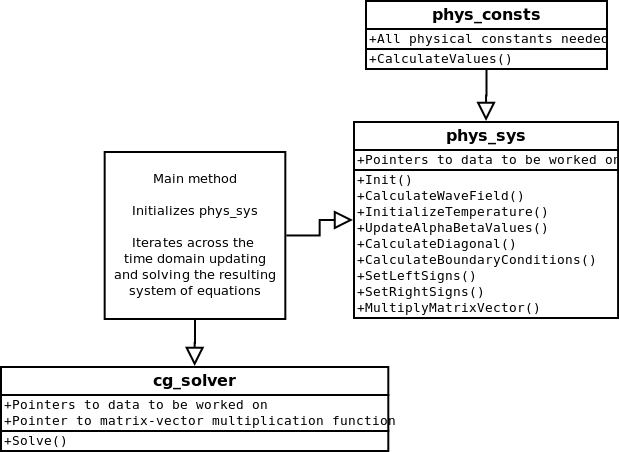
\includegraphics[width=0.5\linewidth]{classdiagram.png}
  \end{center}
  \caption{Class diagram of c++ implementation}
  \label{fig:class_diagram}
\end{figure}


The program mainly consist of three parts:

\begin{itemize}
\item C++ implementation of Linear algebra functionality of the discrete equations.
\item C++ implementation of the conjugate gradient method for solving the
equations described.
\item Bash script for generating plots and and movie of the generated data.
\end{itemize}

The Bash script is not discussed in further detail as it can be considered to be
very simple.

\section{The physical system}

The main task of the physical system is to implement a matrix-vector multiplication
procedure for the heat equation to be used in the conjugate gradient method, 
a method for calculating the heating properties of the microwave and a method 
for calculating the velocity of mass transfer.

\subsection{Partitioning of the problem}

\subsection{Updating alpha and beta values}

Given the temperature, the function UpdateAlphaBeta updates the alpha and beta
values to their correct values by using the temperature to get the current
phase of the substance at each point in the grid.

\subsection{Calculating the distribution of the microwave effect}

This is done according to \cref{eq:effektfordeling} and by multiplying the
resulting distribution by the microwave effect and dividing by the volume at each point
in the grid.

\subsection{The matrix-vector multiplication procedure}

\section{The conjugate gradient method as an iterative algorithm}

\section{The main procedure}

\begin{itemize}

  \item Initialize problem; define grid-size, dimensions of bacon, partitioning of fat vs meat
  and internal and external temperature.
  \item Allocate necessary memory
  \item Initialize physical system
  \item Initialize internal temperature
  \item Initialize internal flow
  \item Calculate boundary conditions
  \item Calculate micro-wave field
  \item Initialize conjugate gradient solver
  \item loop
  \begin{itemize}
    \item Update alpha and beta values
    \item Calculate diagonal
    \item Set signs for right side multiplication (t=n)
    \item Multiply right side of heat equation
    \item Add micro-wave effect to right side of equation
    \item Set signs for left side of equation (t=n+1)
    \item Solve using conjugate gradient method
  \end{itemize}

\item Deallocate memory
\end{itemize}


